\section{Leveleditor}

	\subsection{UML2-Komponentendiagramm}
		\newpage
		\begin{figure}[H]
    		\centering
    		 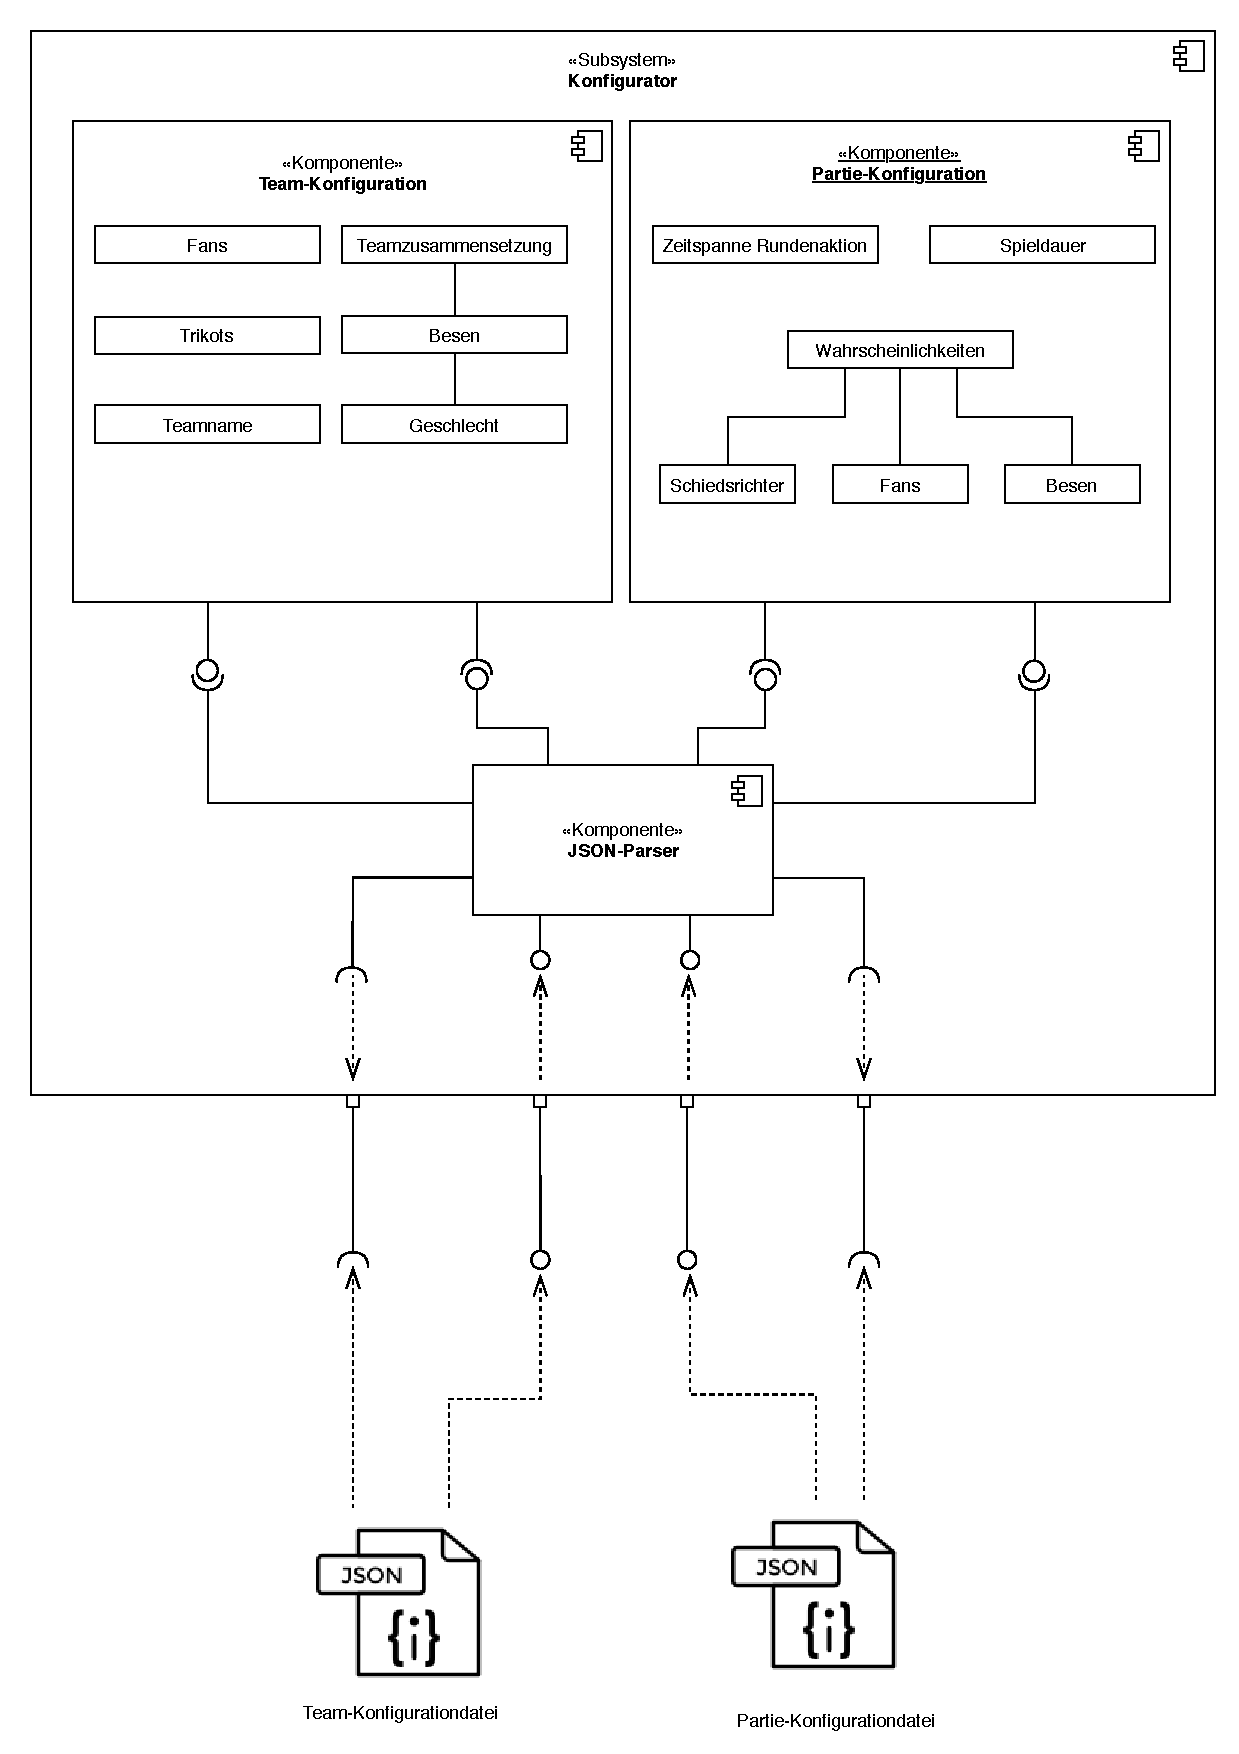
\includegraphics[scale=0.75]{Leveleditor.pdf}
		\end{figure}

	\subsection{Beschreibungen}

		\begin{description}
			
			\item[Konfigurator]
			
			Bei dem Subsystem Konfigurator handelt es sich um eine graphische Benutzeroberfläche, welche zum erstellen von Partie-Konfigurationen, sowie zum erstellen von Team-Konfigurationen  geeignet ist. Der Konfigurator ist lediglich zum erstellen einer gültigen Partie bzw Team-Konfiguration im JSON-Format da, ist aber ein eigenes Programm, und somit unabhängig von den anderen Anwendungen.
			
			\item[Team-Konfiguration]
			Die Team-Konfiguration ist eine der Komponenten, die das Subsystem Konfigurator besitzt. In der Team-Konfiguration kann der Spieler sein Team erstellen, mit seinen gewünschten Parametern. Dies muss der Spieler nur einmal machen und anschliessend kann er seine Konfiguration abspeichern. Ebenso ist die Team-Konfiguration aber auch in der Lage, eine bereits vorhandene Konfiguration zu Laden und diese anschließend zu bearbeiten. Diese Komponente spielt somit eine entscheidende Rolle im Konfigurator, da über sie eine individuelle und gültige Team-Konfiguration erstellt werden kann.
			
			\item[Partie-Konfiguration]
			Die Partie-Konfiguration ist eine Komponente des Subsystems Konfigurator und ist dazu gedacht, dass ein Spieler eine Partie mit seinen gewünschten Einstellungen erstellen kann. In der dafür vorgesehenen graphischen Oberfläche kann der Spieler dann seine Einstellungen leicht einstellen, welche von der Partie-Konfiguration in einem gültigen JSON-Format abgespeichert werden. Die Partie-Konfiguration kann ebenfalls eine bestehende Partie-Konfiguration laden, wo dass diese anschließend bearbeitet werden kann. Die Komponente ist spielt somit eine zentrale Rolle im Subsystem Konfigurator, da über sie erst eine gültige Partie-Konfiguration erstellt werden kann.			
			
			\item[JSON-Parser]
			Der JSON-Parser ist die letzte Komponente des Subsystems Konfigurator und dient dem abspeichern oder Laden der Team, bzw Partie-Konfiguration. Somit stellt der JSON-Parser eine eigene Komponente dar, über die die gewünschten Einstellungen für das Team oder die Partie abgespeichert werden, bzw geladen werden. 

		\end{description}
		
	\subsection{Zuordnung der Funktionalen Anforderungen}
	
	Die funktionalen Anforderungen gemäß dem Pflichtenheft werden den Komponenten folgendermaßen zugeteilt:

	\begin{table}[h]
	\centering
	\begin{tabular}{|l|l|}
		\hline
		\textbf{Komponente} & \textbf{Abgedeckte funktionale Anforderungen}\\ \hline
		Team-Konfiguration & FA53, FA70 \\ \hline
		
		Partie-Konfiguration & FA54, FA70 \\ \hline
		
		JSON-Konverter & FA71, FA72 \\ \hline

	
	\end{tabular}
	\end{table}